\chapter{Using SEXTANTE algorithms}\label{UsingGeoalgorithms}

\section{Introduction. Initial settings}

You can use SEXTANTE geoalgorithms from your application with just a few lines of code. This chapter covers how to use individual algorithms and execute them programmatically, whether from a GIS application or any other application that needs to perform some kind of geospatial analysis.

Don't forget that SEXTANTE also contains graphical elements that can also be integrated into a GIS, incorporating the necessary tools to call geoalgorithms from a graphical user interface. Chapter \ref{IncorporatingGUIElements} covers this topic and shows in detail how to integrate these elements into a GIS. Although those graphical components will take care of calling geoalgorithms and handling their results (which is what we are going to see in this chapter), reading this chapter is recommended before moving to chapter \ref{IncorporatingGUIElements}, since it introduces the fundamental ideas that have to be known before doing any integration with those SEXTANTE elements.

To work through the examples of this chapter you need to follow the following steps to configure you workspace.

First, make sure that your system fulfills the following requirements:

\begin{itemize}
	\item It has a Java 1.6.0 SDK installed \footurl{http://java.sun.com/javase/downloads/index_jdk5.jsp}.
	\item JAI\footurl{https://jai.dev.java.net/binary-builds.html} and JAI Image I/O\footurl{https://jai-imageio.dev.java.net/binary-builds.html} libraries are installed on this SDK.

\end{itemize}

Now, create a new workspace in Eclipse and do the following

\begin{itemize}
 \item Check out the \texttt{geotools\_bindings} folder from the \texttt{sextante\_lib/bindings} folder in the SEXTANTE SVN as a new project in Eclipse. This will download the bindings between SEXTANTE and GeoTools 2.7 and create a project named \texttt{geotools\_bindings}. You can download these bindings also in a jar file from the SEXTANTE website, but in this case we will use the source code directly, since it contains some examples that will be useful and that we will analyze in this chapter.
 \item Download the SEXTANTE core files and put them in a folder named \emph{lib/sextante}, also in the \emph{geotools\_bindings} folder. In the zip file you will also find a folder named \emph{bindings/geotools}. Here is where you can find the jar file with the bindings between SEXTANTE and GeoTools, but, as it has been said, we will not use them.
\item Download GeoTools 2.7 from the GeoTools website\footurl{http://geotools.codehaus.org}. Put all the jar files in a folder named \emph{lib/geotools-2.7.0}, in the \emph{geotools\_bindings} folder. The geotools\_bindings project has SEXTANTE 0.6 jar files and GeoTools jar files already included in its build path. If you are using a different version of SEXTANTE or GeoTools, or you have put those files in a different folder, you will have to change the build path and add the corresponding files instead of the ones already added.

\item Refresh the geotools\_bindings project in your Eclipse IDE.
\end{itemize}

Once you have done this, you already have SEXTANTE, GeoTools and the bindings to link both of them, and also a few examples that we will soon review. Data needed to run this examples can be downloaded from the SEXTANTE website in a single zip file. 

Do not worry if you are not familiar with GeoTools, since we are not going to get deep into it. If you are an advanced GeoTools user, you will be able to make a better use of the library to access your data sources, but if not, the examples just use a few methods that are easy to understand, and are primarily focused on using SEXTANTE, so you should have no problems at all.

Examples are located in the \texttt{es.unex.sextante.geotools.examples} package.

\begin{center}
 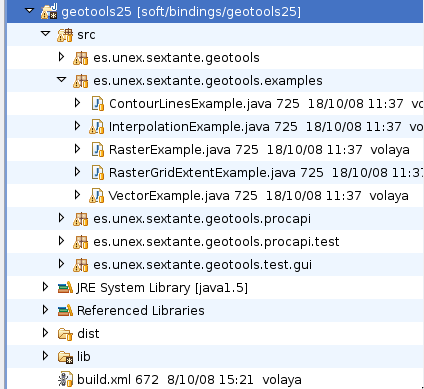
\includegraphics[width=.6\textwidth]{gt_examples.png} 
\end{center}

\section{Executing a geoalgorithm}

Let's open the file named \texttt{VectorExample.java}. This example will open a shapefile containing lines and convert them into points using the \emph{Lines to equispaced points} algorithm in SEXTANTE. The code of the example is fully commented, but for the sake of space we will not copy comments here, but just the fundamental code snippets, showing the main steps that have to be followed to execute a SEXTANTE geoalgorithm.

Here is what you have to do:

\begin{itemize}
\item Initialize the library. That will load the algorithms and start the text engine.

\begin{verbatim}
Sextante.initialize();
\end{verbatim}

\item Wrap you data objects. All data objects used by SEXTANTE (whether as input or as output) must implement the interfaces that were mentioned in the previous chapter. SEXTANTE does not provide a stand--alone implementation of those interfaces, so you have to rely on some geodata library. As it has been said, we will use GeoTools as our data access library.

Let's assume that we have a vector layer in a GeoTools \texttt{DataStore} (In the example, this is done in the \texttt{openShapefile()} method). SEXTANTE cannot understand that object, so we have to wrap it before passing it to the geoalgorithm. The GeoTools bindings include a class named \texttt{GTVectorLayer}, which wraps a \texttt{DataStore} and implements the \texttt{IVectorLayer} interface.

\begin{verbatim}
DataStore ds = ...;
GTVectorLayer layer =GTVectorLayer.createLayer(ds, ds.getTypeNames()[0]);
\end{verbatim}

A \texttt{DataStore} might contain several layers, and this method takes the first layer from the \texttt{DataStore}. The inner base object is not really the \texttt{DataStore} itself, but a \texttt{FeatureStore}.

\texttt{layer} is already an object we can use. We do not need more layers for this example, so let's do something with that layer. 

We create an instance of the algorithm we want to use, in this case an algorithm that converts a line layer into a layer of equispaced points.

\begin{verbatim}
LinesToEquispacedPointsAlgorithm alg = new LinesToEquispacedPointsAlgorithm();
\end{verbatim}

\item Set the input parameters. These parameters can be layers (there we will use the \texttt{GTVectorLayer} that we have created), or simple values such as string or numerical ones. In this case we need to set an input layer and a distance between points.

\begin{verbatim}
ParametersSet params = alg.getParameters();
params.getParameter(LinesToEquispacedPointsAlgorithm.LINES)
                      .setParameterValue(layer);
params.getParameter(LinesToEquispacedPointsAlgorithm.DISTANCE)
                      .setParameterValue(new Double(5000));
\end{verbatim}

The \texttt{ParametersSet} class represents a parameter container, and each algorithm has an object of this class that you can get using the \texttt{getParameters()} method.

\item Create an output factory. Output factories tell SEXTANTE how to create new data objects. These new data object will also implement the corresponding SEXTANTE interfaces (that means that, for instance, a vector layer will implement the IVectorLayer interface that we already know).

Once again, SEXTANTE does not provide a standalone output factory, but there are several ones already developed, each one of them based on some geodata library. The \texttt{GTOutputFactory} included in the GeoTools binding generates objects based on GeoTools data objects.

\begin{verbatim}
 OutputFactory outputFactory = new GTOutputFactory();
\end{verbatim}

Using this factory means that the algorithm will create wrapped GeoTools objects as output layers.

\item Set the output filenames. The outputs generated by the algorithm using the output factory are file--based (particularly, in this case it generates shapefiles), so a filename is needed. If you don't set one, the output factory will create a temporary filename. Some output factories might not use that filename, for example if they store everything in memory.

\begin{verbatim}
OutputObjectsSet outputs = alg.getOutputObjects();
Output contours = outputs.getOutput(LinesToEquispacedPointsAlgorithm.RESULT);
contours.setFilename("/home/my_user_name/points.shp");
\end{verbatim}

\item Execute the algorithm. We pass the output factory to the algorithm, so it knows how to create the resulting objects. The first parameter is an object implementing the \texttt{ITaskMonitor} interface, used to monitor the activity of the algorithm. If we pass a null value, then it will use a silent monitor. SEXTANTE provides a \texttt{DefaultTaskMonitor} as well, which just shows a simple Java progress monitor with a cancel button.

\begin{verbatim}
alg.execute(null, outputFactory);
\end{verbatim}

\item Get the results. The \texttt{OutputObjectsSet} class used to retrieve the outputs and set the filename for each of them (see last point) can be used to get the resulting data as well. The \texttt{Output} object that we retrieved contained a null object then, but now it should have been replaced by a valid output object.

\begin{verbatim}
 IVectorLayer result = (IVectorLayer) contours.getOutputObject();
\end{verbatim}

Since we used a\texttt{GTOutputFactory}, it will be a \texttt{GTVectorLayer} object. We can take the internal base data object it is based on, which in this case will be a GeoTools \texttt{FeatureStore}

\begin{verbatim}
 FeatureStore fs = (FeatureStore) result.getBaseDataObject();
\end{verbatim}

\end{itemize}

And now we have a resulting object and we have succesfully used a SEXTANTE geoalgorithm.

Let's try now another another algorithm, in this case one that works with raster layers. Open the \texttt{RasterGridExtentExample}. This is the code of its \texttt{doProcessing()} method, where all the actual processing takes place:

\begin{verbatim}
GridCoverage2D gc = openRasterLayer("/home/my_user_name/dem.asc");
GTRasterLayer dem = new GTRasterLayer();
dem.create(gc);

SlopeAlgorithm alg = new SlopeAlgorithm();
ParametersSet params = alg.getParameters();
params.getParameter(SlopeAlgorithm.DEM).setParameterValue(dem);

params.getParameter(SlopeAlgorithm.METHOD).setParameterValue(
                        SlopeAlgorithm.METHOD_ZEVENBERGEN);

params.getParameter(SlopeAlgorithm.UNITS).setParameterValue(
                        SlopeAlgorithm.UNITS_RADIANS);

OutputObjectsSet outputs = alg.getOutputObjects();
Output out = outputs.getOutput(SlopeAlgorithm.SLOPE);
out.setFilename("/home/my_user_name/slope.tif");

AnalysisExtent ge = dem.getLayerGridExtent();
ge.setCellSize(100.);
alg.setAnalysisExtent(ge);

alg.execute(null, m_OutputFactory);

IRasterLayer slope = (IRasterLayer) out.getOutputObject();

System.out.println("The output cellsize is "
                 + Double.toString(slope.getLayerGridExtent().getCellSize())
                 + " m");
\end{verbatim}

Most of the code looks quite similar to the one in the vector example, and it follows the steps described above. This time, a \texttt{GridCoverage2D} is used as the base data object, and it is wrapped with a \texttt{GTRasterLayer} object, since it is a raster layer instead of a vector one.

The main difference, however, is found just before the algorithm execution, in the lines shown next.

\begin{verbatim}
AnalysisExtent ge = dem.getLayerGridExtent();
ge.setCellSize(100.);
alg.setAnalysisExtent(ge);
\end{verbatim}

Whenever a SEXTANTE geoalgorithm generates new layers, the extent (and cellsize if it is a raster layer) of the resulting layers can be selected before executing the algorithm. Using this, you can, for instance, take a raster layer covering a large area as the input of a geoalgorithm, and generate output layers that cover just a small part of that area and not necessarily all of it. If you do not explicitly set the characteristics of output layers, SEXTANTE will infere them from input layers. In this case, since there is only a single input raster layer, commenting out the above three lines will cause the resulting slope layer to have the same characteristics as the input DEM.

Some algorithms do not allow the user to select the analysis extent used to analize input layers and generate new ones. In that case, calling the \texttt{setAnalysisExtent} method makes no difference at all, since the algorithm is not going to use the information provided through that method.

To set the characteristics of output layers, the \texttt{setAnalysisExtent(AnalysisExtent)} method has to be used. An \texttt{AnalysisExtent} contain information about the extent and the cellsize to use (even if the algorithm deals only with vector layers, the \texttt{AnalysisExtent} has a cell size, though it is not used), and also some additional methods to handle and create this information.

In the proposed example, the extent of the input DEM is taken (all object of class \texttt{IRasterLayer} have one, a copy of which can be retrieved using the \texttt{getLayerGridExtent()} method), and its cellsize changed to 100. The original cellsize of the input DEM is 25 meters, so we are telling SEXTANTE to create a resulting layer with a coarser resolution.

In some cases, setting the analysis extent is mandatory, since there are algorithms that generate layers but do not take other layers of that kind as input. This happens, for instance, in all the interpolation algorithms. In the \texttt{InterpolationExample} class you will find the following code:

\begin{verbatim}
AnalysisExtent extent = new AnalysisExtent(layer);
extent.setCellSize(25.);
alg.setAnalysisExtent(extent);
\end{verbatim}

A new \texttt{AnalysisExtent} object is created, passing a layer (a vector layer in this case) to the constructor. The full extent (the area to cover) of the vector layer is used, but since vector layers do not have a cellsize value, the cellsize must be set manually afterwards. 

In this case, commenting out these lines will cause the algorithm to throw an exception when executed, since it will not have enough information to produce any output (the cellsize of the ouput layer cannot be taken from the input layer, since the latter is a vector one, and vector layers do not have a cellsize value).

